\documentclass[12pt]{article}
\usepackage{amsmath}
\usepackage{amssymb}
\usepackage{geometry}
\usepackage{enumerate}
\usepackage{natbib}
\usepackage{float}%稳定图片位置
\usepackage{graphicx}%画图
\usepackage[english]{babel}
\usepackage{a4wide}
\usepackage{indentfirst}%缩进
\usepackage{enumerate}%加序号
\usepackage{multirow}%合并行


\begin{document}
\newpage
\section{Problem 2}
\subsection{(a)}
\subsubsection{(i)}
When $V_{gs}=1V$, we get the figure
\begin{figure}[H]
\centering
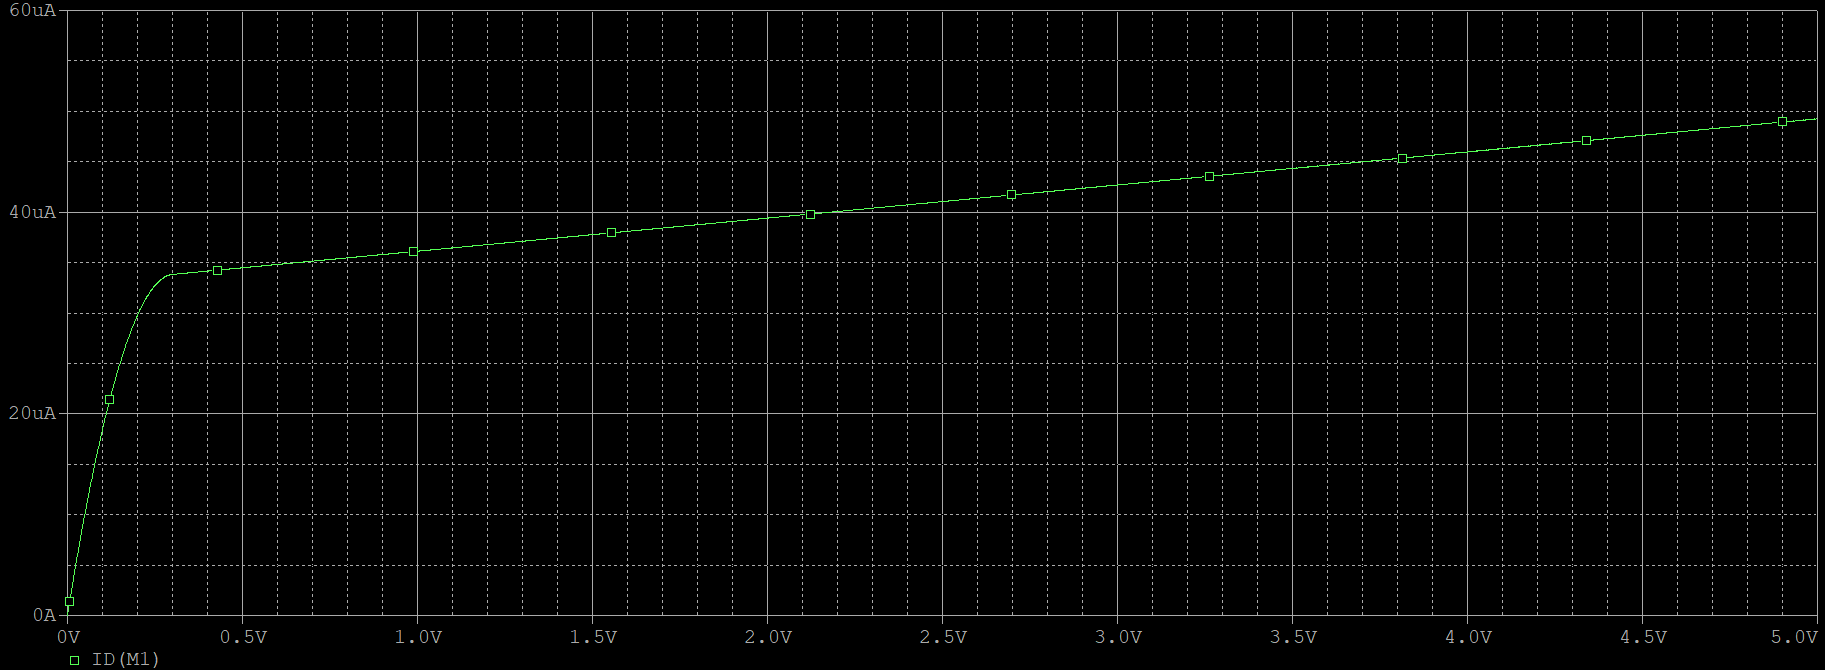
\includegraphics[scale=0.23]{P1.png}
\end{figure}
From the figure we know that when $V_d<0.3V$, it's in triode region and when $V_d>0.3V$, its' in saturation region. The slope is $\frac{15.15\cdot10^{-6}}{4.6}=3.27\cdot10^{-6}$, so $R_0=\frac{1}{slope}=3.06\cdot10^{6}\Omega$
$$I_d=0.5\mu_nC_{ox}\frac{W}{L}(V_{GS}-V_{TH})^2=0.5*0.035*\frac{3.9*8.85*10^{-12}}{9*10^{-9}}*\frac{10}{2-2*0.08}*(1-0.7)^2=3.26\cdot10^{-5}$$
$$r_0=\frac{1}{I_d*\lambda}=\frac{1}{3.26\cdot10^{-6}}=306667\Omega$$
\subsubsection{(ii)}
When $V_{gs}=1.5V$, we get the figure
\begin{figure}[H]
\centering
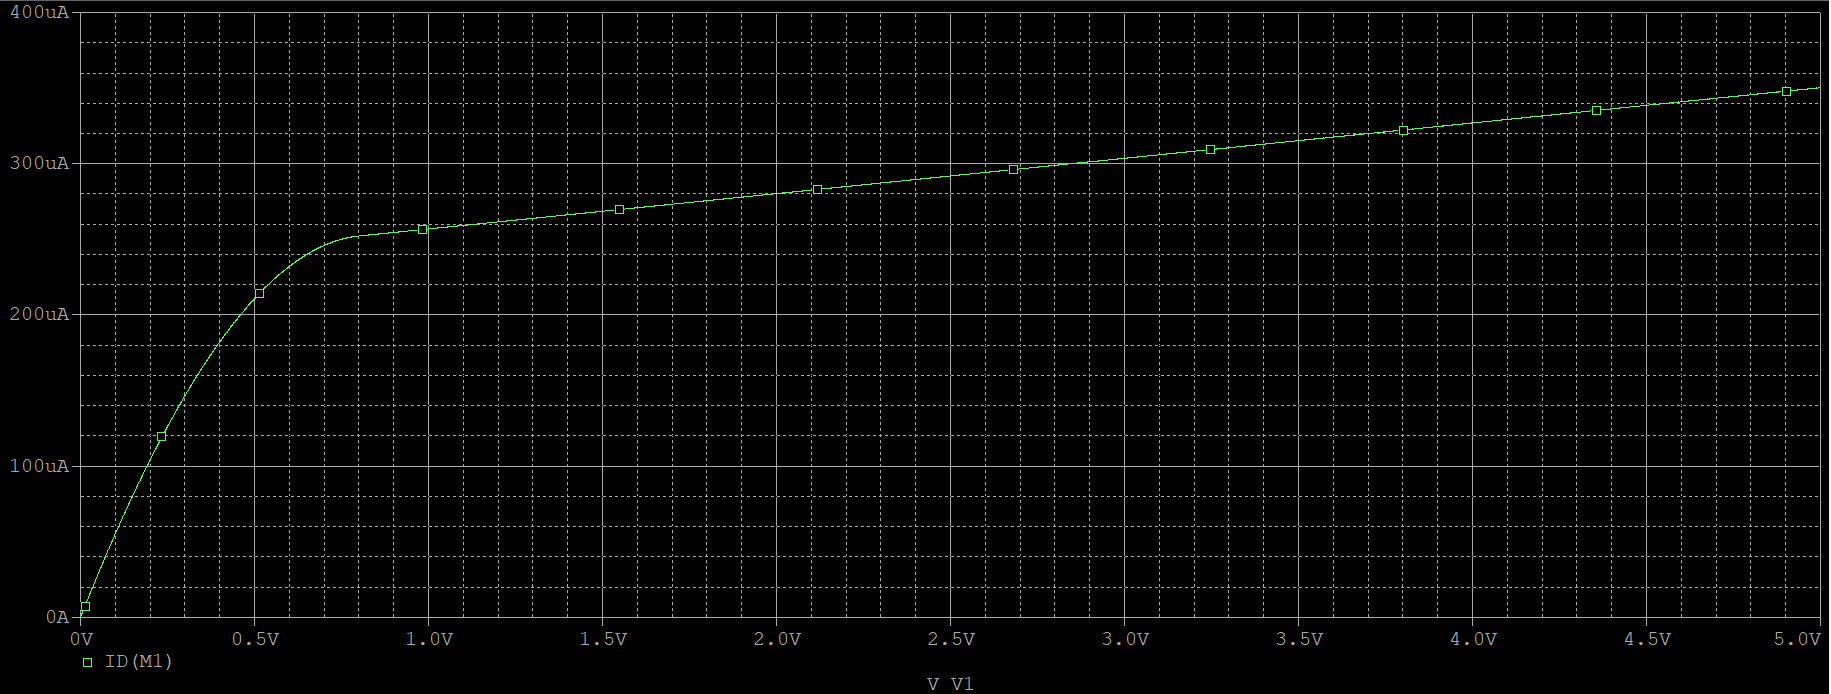
\includegraphics[scale=0.23]{P2.png}
\end{figure}
From the figure we know that when $V_d<0.8V$, it's in triode region and when $V_d>0.8V$, its' in saturation region. The slope is $\frac{97.8\cdot10^{-6}}{4.1}=2.39\cdot10^{-5}$, so $R_0=\frac{1}{slope}=4.19\cdot10^{4}\Omega$
$$I_d=0.5\mu_nC_{ox}\frac{W}{L}(V_{GS}-V_{TH})^2=0.5*0.035*\frac{3.9*8.85*10^{-12}}{9*10^{-9}}*\frac{10}{2-2*0.08}*(1.5-0.7)^2=2.32\cdot10^{-4}$$
$$r_0=\frac{1}{I_d*\lambda}=\frac{1}{2.32\cdot10^{-5}}=43192\Omega$$
\subsubsection{(iii)}
When $V_{gs}=2V$, we get the figure
\begin{figure}[H]
\centering
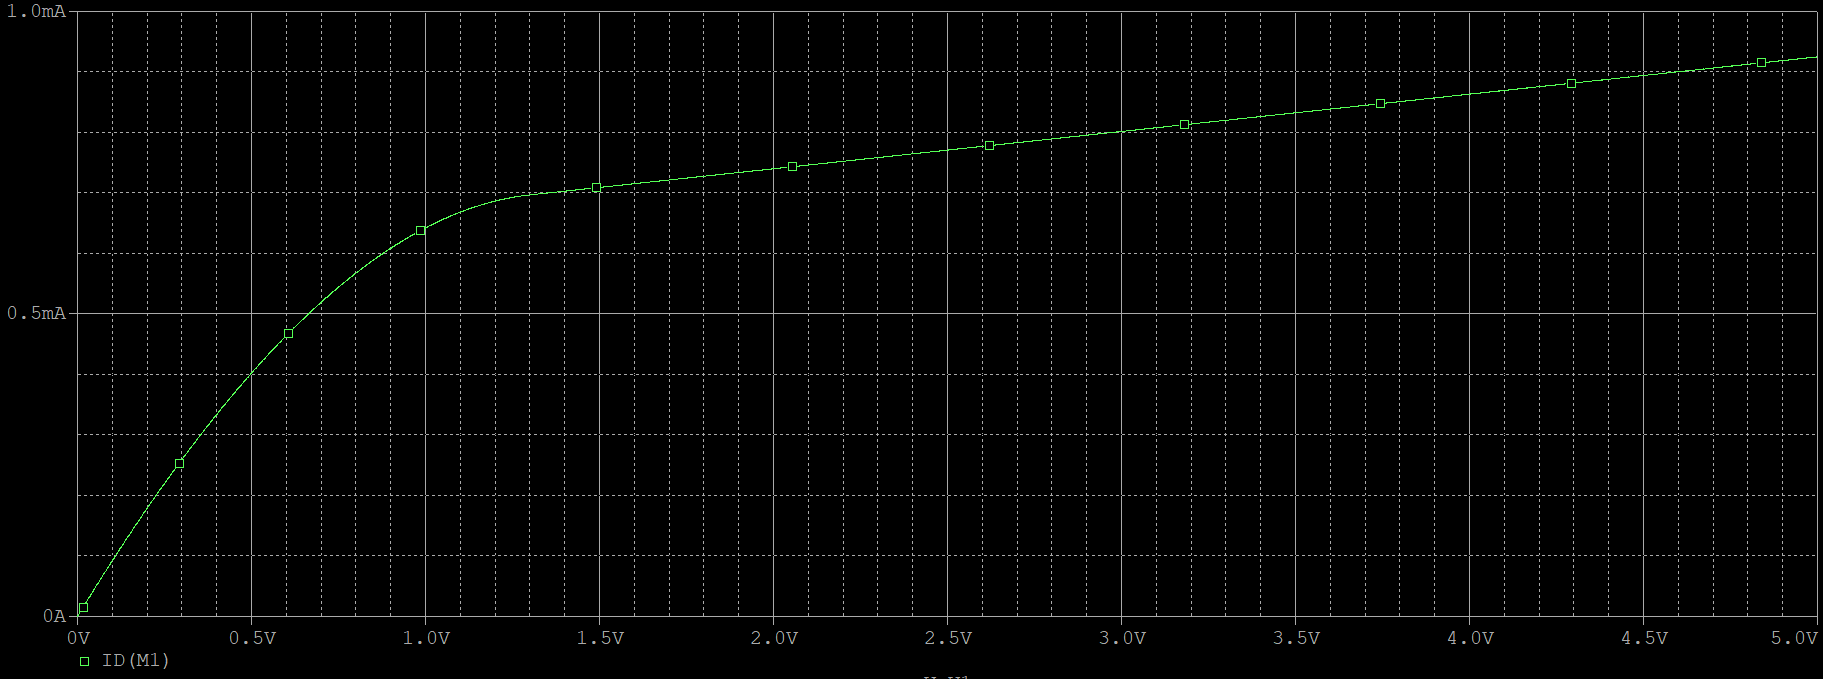
\includegraphics[scale=0.23]{P3.png}
\end{figure}
From the figure we know that when $V_d<0.8V$, it's in triode region and when $V_d>0.8V$, its' in saturation region. The slope is $\frac{227.7\cdot10^{-6}}{3.7}=6.15\cdot10^{-5}$, so $R_0=\frac{1}{slope}=1.62\cdot10^{4}\Omega$
$$I_d=0.5\mu_nC_{ox}\frac{W}{L}(V_{GS}-V_{TH})^2=0.5*0.035*\frac{3.9*8.85*10^{-12}}{9*10^{-9}}*\frac{10}{2-2*0.08}*(2-0.7)^2=6.16\cdot10^{-4}$$
$$r_0=\frac{1}{I_d*\lambda}=\frac{1}{6.16\cdot10^{-5}}=16226\Omega$$
All my calculated $r_o$ are a little bigger than the simulated one.
\subsection{(b)}
\begin{figure}[H]
\centering
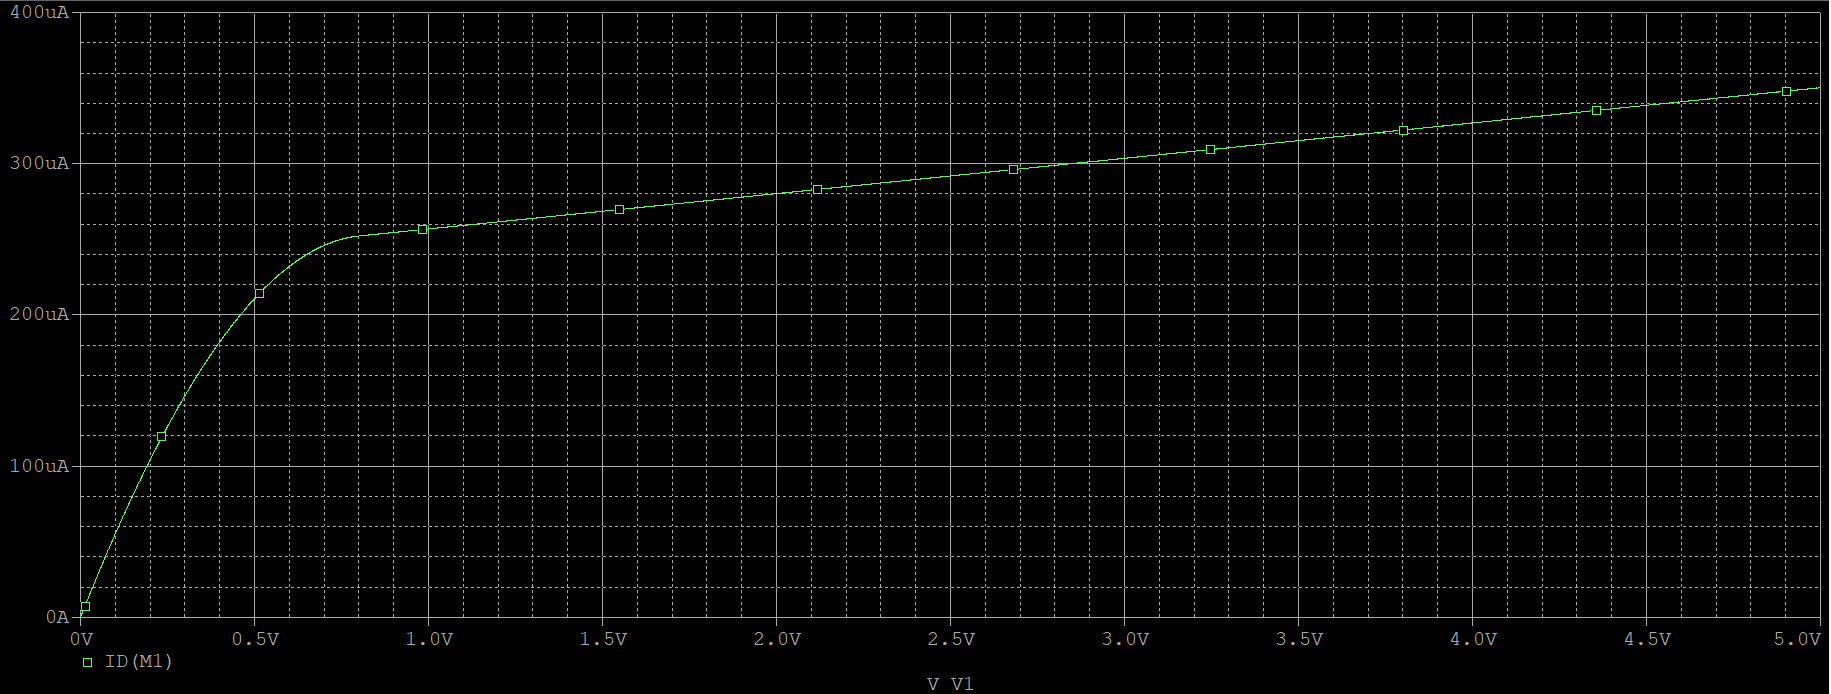
\includegraphics[scale=0.23]{P2.png}
\end{figure}
The slope is $\frac{30\cdot10^{-6}}{20\cdot10^{-3}}=1.5\cdot10^{-3}$
$$gm=\mu_nC_{ox}\frac{W}{L}(V_{GS}-V_{TH})*(1+\lambda V_{DS})=0.035*\frac{3.9*8.85*10^{-12}}{9*10^{-9}}*5*(2-0.7)*(1+0.1*5)=1.3\cdot10^{-3}(\Omega^{-1})$$
My calculated values are very close to the simulated values.
\end{document}